%%%%%%%%%%%%%%%%%%%%%%%%%%%%%%%%%%%%%%%%%%%%%%%%%%%%%%%%%%%%%%%%%
%% 
%% IT Project Report template, v0.2
%% 
%% INSTRUCTIONS FOR COMPILING THIS DOCUMENT (using GNU/Linux command line)
%% 
%% pdflatex it-report.tex; bibtex it-report.aux
%% 
%%%%%%%%%%%%%%%%%%%%%%%%%%%%%%%%%%%%%%%%%%%%%%%%%%%%%%%%%%%%%%%%%

\documentclass[oneside,a4paper,11pt]{report}

%%%%%%%%%%%%%%%%%%%%%%%%%%%%%%%%%%%%%%%%%%%%%%%%%%%%%%%%%%%%%%%%%
%% PREAMBLE.
%%%%%%%%%%%%%%%%%%%%%%%%%%%%%%%%%%%%%%%%%%%%%%%%%%%%%%%%%%%%%%%%%

%%%%%%%%%%%%%%%%%%%%%%%%%%%%%%%%%%%%%%%%%%%%%%%%%%%%%%%%%%%%%%%%%
%% ANOTHER LATEX THESIS TEMPLATE.
%% https://github.com/zachscrivena/another-latex-thesis-template
%% This is free and unencumbered software released into the
%% public domain; see <http://unlicense.org> for details.
%%%%%%%%%%%%%%%%%%%%%%%%%%%%%%%%%%%%%%%%%%%%%%%%%%%%%%%%%%%%%%%%%



%%%%%%%%%%%%%%%%%%%%%%%%%%%%%%%%%%%%%%%%%%%%%%%%%%%%%%%%%%%%%%%%%
%% PAGE SIZE AND MARGINS.
%%%%%%%%%%%%%%%%%%%%%%%%%%%%%%%%%%%%%%%%%%%%%%%%%%%%%%%%%%%%%%%%%

% Letter-size (8.5in x 11in) single-sided pages,
% with margins (top,right,bottom,left) = (1,1,1,1.5)in,
% and header 0.25in above the text body.
\usepackage[
	paper=a4paper, % Default paper size, change to "letterpaper" for US Letter (you'll need to adjust margins after)
	inner=1.5in, % The inner margin (beside binding)
	outer=1in, % The outer margin (opposite binding)
	top=.8in, % Top margin
	bottom=.7in, % bottom margin
	headheight=20pt, % Header height
	headsep=.25in, % Header separation
	includehead,
	includefoot]{geometry}

%%%%%%%%%%%%%%%%%%%%%%%%%%%%%%%%%%%%%%%%%%%%%%%%%%%%%%%%%%%%%%%%%
%% COLORS.
%%%%%%%%%%%%%%%%%%%%%%%%%%%%%%%%%%%%%%%%%%%%%%%%%%%%%%%%%%%%%%%%%
\usepackage[usenames]{color} % For colors.

%%%%%%%%%%%%%%%%%%%%%%%%%%%%%%%%%%%%%%%%%%%%%%%%%%%%%%%%%%%%%%%%%
%% MISCELLANEOUS PACKAGES.
%%%%%%%%%%%%%%%%%%%%%%%%%%%%%%%%%%%%%%%%%%%%%%%%%%%%%%%%%%%%%%%%%

\usepackage{graphicx}
\usepackage[utf8]{inputenc}
\usepackage[english]{babel} % For language-specific hyphenation.
%\usepackage{polski}
\usepackage{cite} % Automatically sort and range citations numbers.
\usepackage{environ} % For easy definition of environments.
\usepackage{rotating} % For rotating objects.
\usepackage{framed} % For framed text.
\usepackage{enumitem}
\usepackage{longtable}
\usepackage{placeins}
\usepackage{lipsum}

%\hyphenation{dźwię-ku}

\usepackage{subfig}
\usepackage{tikz}
\usetikzlibrary{shapes,arrows,chains,decorations.markings,calc,shapes.geometric,intersections}
\usetikzlibrary{decorations.pathmorphing}
\usepackage{tkz-euclide}
%\usetkzobj{all}

\usepackage{longtable}
\usepackage{array}
\usepackage{multicol}
\newcommand{\inches}{$\mathrm{^{\prime\prime}}$}

\graphicspath{
	{Figures/}
		{./}
}

\newcommand{\todo}{\mbox{\color{red} TODO!}}



%%%%%%%%%%%%%%%%%%%%%%%%%%%%%%%%%%%%%%%%%%%%%%%%%%%%%%%%%%%%%%%%%
%% PDF OUTPUT.
%%%%%%%%%%%%%%%%%%%%%%%%%%%%%%%%%%%%%%%%%%%%%%%%%%%%%%%%%%%%%%%%%

% PDF settings and properties (set options with \hypersetup{}).
\usepackage{hyperref} % For TEX --> DVI --> PDF.
% \usepackage[pdftex]{hyperref} % For TEX --> PDF.

%%%%%%%%%%%%%%%%%%%%%%%%%%%%%%%%%%%%%%%%%%%%%%%%%%%%%%%%%%%%%%%%%
%% FONTS.
%%%%%%%%%%%%%%%%%%%%%%%%%%%%%%%%%%%%%%%%%%%%%%%%%%%%%%%%%%%%%%%%%

\usepackage[T1]{fontenc}
\usepackage{lmodern} % For Latin Modern fonts.
\usepackage{times}

% Sans-serif fonts.
\usepackage[scaled=0.89]{helvet}
\renewcommand{\sffamily}{\usefont{T1}{phv}{m}{n}}
\newcommand{\UseLMSSBoldFont}{\usefont{T1}{lmss}{m}{n}\bfseries}

% Monospace (typewriter) font.
\usepackage[scaled=0.78]{beramono}
\renewcommand{\ttfamily}{\usefont{T1}{fvm}{m}{n}}

%%%%%%%%%%%%%%%%%%%%%%%%%%%%%%%%%%%%%%%%%%%%%%%%%%%%%%%%%%%%%%%%%
%% SECTION HEADINGS.
%%%%%%%%%%%%%%%%%%%%%%%%%%%%%%%%%%%%%%%%%%%%%%%%%%%%%%%%%%%%%%%%%

% Section heading fonts.
\usepackage{sectsty} % For selecting fonts for section headings.
\allsectionsfont{\UseLMSSBoldFont}

% Section numbering depth.
\setcounter{secnumdepth}{10}

%%%%%%%%%%%%%%%%%%%%%%%%%%%%%%%%%%%%%%%%%%%%%%%%%%%%%%%%%%%%%%%%%
%% PARAGRAPHS.
%%%%%%%%%%%%%%%%%%%%%%%%%%%%%%%%%%%%%%%%%%%%%%%%%%%%%%%%%%%%%%%%%

% Line spacing.
\usepackage{setspace}
%\singlespacing
%\onehalfspacing
%\doublespacing
\setstretch{1.35} % custom

% Indented blocks.
\newcommand{\IndentBlock}[1]{\noindent\hangafter=0\hangindent=#1\parindent\ignorespaces}
\newcommand{\IndentHanging}{\noindent\hangafter=1\hangindent=\parindent\ignorespaces}

\usepackage{indentfirst}

%%%%%%%%%%%%%%%%%%%%%%%%%%%%%%%%%%%%%%%%%%%%%%%%%%%%%%%%%%%%%%%%%
%% HEADERS AND FOOTERS.
%%%%%%%%%%%%%%%%%%%%%%%%%%%%%%%%%%%%%%%%%%%%%%%%%%%%%%%%%%%%%%%%%
% \includegraphics[height=0.5in]{ue.jpg}}
% Header.
\usepackage{fancyhdr}

\fancypagestyle{empty}{%
	\fancyhf{}
	\fancyhead[L]{\parbox[b]{20mm}{}}
	\fancyhead[R]{\parbox[b]{48mm}{}}
	\renewcommand{\headrulewidth}{0.0pt}
	\renewcommand{\footrulewidth}{0.0pt}}

\fancypagestyle{regular}{%
	\fancyhf{}
	\fancyfoot[C]{\thepage}
	\fancyhead[L]{\parbox[b]{20mm}{}}
	\fancyhead[R]{\parbox[b]{48mm}{}}
	\renewcommand{\headrulewidth}{0.0pt}
	\renewcommand{\footrulewidth}{0.0pt}}

\fancypagestyle{plain}{%
	\fancyhf{}
	\fancyhead[L]{\parbox[b]{20mm}{}}
	\fancyhead[R]{\parbox[b]{48mm}{}}
	\fancyfoot[C]{\thepage}
	\renewcommand{\headrulewidth}{0.0pt}
	\renewcommand{\footrulewidth}{0.0pt}}

\pagestyle{regular}

%%%%%%%%%%%%%%%%%%%%%%%%%%%%%%%%%%%%%%%%%%%%%%%%%%%%%%%%%%%%%%%%%
%% FOOTNOTES.
%%%%%%%%%%%%%%%%%%%%%%%%%%%%%%%%%%%%%%%%%%%%%%%%%%%%%%%%%%%%%%%%%

% Blank footnotes.
\newcommand\BlankFootnote[1]{%
	\begingroup%
	\renewcommand{\thefootnote}{}%
	\footnotetext{#1}%
	\addtocounter{footnote}{-1}%
	\addtocounter{Hfootnote}{-1}%
	\endgroup}

%%%%%%%%%%%%%%%%%%%%%%%%%%%%%%%%%%%%%%%%%%%%%%%%%%%%%%%%%%%%%%%%%
%% LISTS.
%%%%%%%%%%%%%%%%%%%%%%%%%%%%%%%%%%%%%%%%%%%%%%%%%%%%%%%%%%%%%%%%%

% Numbered lists in IEEE style.
% (Individual lists can be modified by redefining
% these macros inside the enumerate environment.)
\makeatletter
% 1st level: 1), 2), 3)
\renewcommand{\theenumi}{\arabic{enumi}}
\renewcommand{\labelenumi}{\theenumi)}
% 2nd level: a), b), c)
\renewcommand{\theenumii}{\alph{enumii}}
\renewcommand{\labelenumii}{\theenumii)}
\renewcommand\p@enumii{}
% 3rd level: i), ii), iii)
\renewcommand{\theenumiii}{\roman{enumiii}}
\renewcommand{\labelenumiii}{\theenumiii)}
\renewcommand\p@enumiii{}
% 4th level: A), B), C)
\renewcommand{\theenumiv}{\Alph{enumiv}}
\renewcommand{\labelenumiv}{\theenumiv)}
\renewcommand\p@enumiv{}
\makeatother

% Definition items.
\newcommand{\DefineItem}[1]{%
	\IndentBlock{1}#1\nopagebreak
	\par\IndentBlock{2}}


%%%%%%%%%%%%%%%%%%%%%%%%%%%%%%%%%%%%%%%%%%%%%%%%%%%%%%%%%%%%%%%%%
%% FIGURES AND TABLES.
%%%%%%%%%%%%%%%%%%%%%%%%%%%%%%%%%%%%%%%%%%%%%%%%%%%%%%%%%%%%%%%%%

\usepackage{graphicx} % To support graphics in EPS format.
\usepackage{multirow} % To support multi-row cells in tables.
\usepackage{booktabs} % For making nice tables.

% Adjust spacing between table rows.
\renewcommand*\arraystretch{1.25}

% Dashed lines in tables.
\usepackage{arydshln}
\def\dashvertical{;{2pt/3pt}}
\def\dashhorizontal{\hdashline[2pt/3pt]}

% Captions for figures and tables.
\newcommand{\CaptionFontSize}{\small}

\makeatletter
\def\@figurestring{figure}
\def\@tablestring{table}
\def\@makecaption#1#2{%
	\CaptionFontSize
	\ifx\@captype\@figurestring
		\vskip1em
	\fi
	\sbox\@tempboxa{{\sffamily\bfseries{#1.}}\hspace{0.5em}#2}%
	\ifdim\wd\@tempboxa>\hsize
		{{\sffamily\bfseries{#1.}}\hspace{0.5em}#2}%
	\else
		\hb@xt@\hsize{\hfil\box\@tempboxa\hfil}%
	\fi
	\ifx\@captype\@tablestring
		\vskip1em
	\fi
}
\makeatother


%% \definecolor{MyDarkBlue}{rgb}{0,0.08,0.45}
%% {\color{MyDarkBlue}This text is dark blue}

%%%%%%%%%%%%%%%%%%%%%%%%%%%%%%%%%%%%%%%%%%%%%%%%%%%%%%%%%%%%%%%%%
%% DATE AND TIME.
%%%%%%%%%%%%%%%%%%%%%%%%%%%%%%%%%%%%%%%%%%%%%%%%%%%%%%%%%%%%%%%%%

\usepackage{datetime} % For dates and times.
\renewcommand{\dateseparator}{-}
\settimeformat{xxivtime}

% Timestamp.
\newcommand{\Timestamp}{{\yyyymmdddate\today}~{\currenttime}}


%%%%%%%%%%%%%%%%%%%%%%%%%%%%%%%%%%%%%%%%%%%%%%%%%%%%%%%%%%%%%%%%%
%% MATHEMATICS.
%%%%%%%%%%%%%%%%%%%%%%%%%%%%%%%%%%%%%%%%%%%%%%%%%%%%%%%%%%%%%%%%%

\usepackage{amsmath,amsfonts,amsbsy,amsthm} % AMS packages.



%%%%%%%%%%%%%%%%%%%%%%%%%%%%%%%%%%%%%%%%%%%%%%%%%%%%%%%%%%%%%%%%%
%% TABLE OF CONTENTS (TOC) SETTINGS.
%%%%%%%%%%%%%%%%%%%%%%%%%%%%%%%%%%%%%%%%%%%%%%%%%%%%%%%%%%%%%%%%%

% TOC depth.
\setcounter{tocdepth}{10}

% Suppress entries in the TOC.
\newcommand{\DummyThree}[3]{}

\newcommand{\DisableTOCUpdates}{%
	\let\tempaddcontentsline=\addcontentsline
	\let\addcontentsline=\DummyThree}

\newcommand{\EnableTOCUpdates}{%
	\let\addcontentsline=\tempaddcontentsline}


\usepackage{lipsum} % For sample/blind text.





%%%%%%%%%%%%%%%%%%%%%%%%%%%%%%%%%%%%%%%%%%%%%%%%%%%%%%%%%%%%%%%%%
%% ACTUAL DOCUMENT.
%%%%%%%%%%%%%%%%%%%%%%%%%%%%%%%%%%%%%%%%%%%%%%%%%%%%%%%%%%%%%%%%%

\begin{document}

% Use Roman numerals (i, ii, iii, etc.) for page numbers.
% \pagenumbering{roman}

%%%%%%%%%%%%%%%%%%%%%%%%%%%%%%%%%%%%%%%%%%%%%%%%%%%%%%%%%%%%%%%%%
%% TITLE PAGE.
%%%%%%%%%%%%%%%%%%%%%%%%%%%%%%%%%%%%%%%%%%%%%%%%%%%%%%%%%%%%%%%%%

% No headers or footers on the title page.
\thispagestyle{empty}

\begin{titlepage}
    {\centering
        \setstretch{1.0}
        \null
        \vspace{-1.0in}
        
\includegraphics[width=1.8in]{polsl_logo2_zn_en.pdf}\\[2.5em]
        \normalfont\LARGE
        Faculty of Automatic Control, \\Electronics and Computer Science \\[1.3em]
        \normalfont\LARGE
        Internet Technologies -- project work \\[1.5em]
        \UseLMSSBoldFont\LARGE
        Cyberventure game\\[5.2em]}
    \normalfont\large
    \noindent
    Authors:
    \\[0.5em]
    Mateusz Siedliski\\
    Radosław Tchórzewski
    \\[1.5em]
    Year 2022/2023, semester 5, group 6, section 9:
    \\[0.5em]
    Project supervisor: mgr inż. Oliwia Krauze
    \\[1.5em]

    \vfill
    \centering Gliwice 2023
    \par
\end{titlepage}




\pagestyle{plain}
% \setcounter{page}{2}


% \clearpage



%%%%%%%%%%%%%%%%%%%%%%%%%%%%%%%%%%%%%%%%%%%%%%%%%%%%%%%%%%%%%%%%%
%% TABLE OF CONTENTS (TOC), LISTS OF FIGURES/TABLES/ETC.
%%%%%%%%%%%%%%%%%%%%%%%%%%%%%%%%%%%%%%%%%%%%%%%%%%%%%%%%%%%%%%%%%

\tableofcontents

%\listoffigures

%\listoftables

% \clearpage


% Use Arabic numerals (1, 2, 3, etc.) for page numbers.
\pagenumbering{arabic}




\chapter{Introduction}
When "Flappy Bird" came out in 2013, it has brought a lot of attention. There were reports of people breaking their devices, thanks to the rage caused by difficult gameplay. The game concept was simple. Try to avoid obstacles moving forward by tapping the screen to go up while gravity constantly pulls you down.

\par
We've decided to create a new and improved version of this game. During our project we've explored new fitting and interesting graphic designs. We've used many languages and technologies we haven't used before, which was made possible thanks to the web developer bootcamp we took \cite{Bootcamp}. Our game contains features such as adding additional pickups, laser meant to be avoided and gravity switching. We were aiming to create a feeling of fair gameplay with options that reminded us of flash games hosted on various websites, and we think we've managed to achieve that. Gaining knowledge about which tools we have to use was vastly improved thanks to the
YouTube's tutorials \cite{CodingTrain} \cite{Phpcourse} \cite{ProgrammingwithMosh}.

\par
Although many versions of "Flappy Bird" were created, none of them seemed to change the concept enough. We've created an experience that is unique thanks to the graphic design and challenging in a fair way without encouraging anger. We wanted to give players an additional sense of challenge by implementing a global leaderboard.

\chapter{Aim and scope of the project}

Our game consists of two distinct parts: client side website and server with MySQL database responsible for providing global leaderboard. A player can see top 5 scores of the best players, as well as the highest score from the current session and current score for the round. A JavaScript structure based on p5.js library is responsible for handling rendering assets\cite{Blender} and preparing each frame. We needed jQuery library to communicate between client and server side. The game is hosted on free external hosting.

\par
We've decided to use p5.js library as our main starting point. Furthermore, we made this decision knowing that this library contains powerful tools for creating looping graphics and rendering images on website correctly. A second library called jQuery was chosen for its event handling, animation and Ajax handling.

\par
MySQL was chosen as our database system thanks to it being free and having easy to use interface. To prevent overfilling the database we've used a job scheduler called cron.


\chapter{Schedule}
\section{Schedule approved at the beginning}
\begin{itemize}
	\item Learning HTML and creating 1st version of homepage
	\item Learning CSS and creating styles for the webpage
	\item Learning JavaScript and creating first sketch of the game
	\item Creating game physics (collision)
	\item Learning PHP and creating simple communication between website and the database for storing high scores
	\item Adding Leaderboard and accounts system
	\item Adding collectibles/game speed mechanic
	\item Implementing dynamic background (changed by earning more points, constantly moving behind player to give impression of speed)
	\item Creating final graphics, sprites and finalizing project
\end{itemize}

\newpage

\section{Schedule reflecting actual work}
\begin{itemize}
	\item Learning HTML and creating 1st version of homepage
	\item Learning CSS and experimenting with styles (made temporary ones)
	\item Learning JavaScript and creating first sketch of the game
	\item Creating game physics (collision) and implementing temporary sprites
	\item Reworking background rendering and collision to optimize code
	\item Learning PHP and creating communication between website and the database for storing players scores. Adding user input after game is ended.
	\item Implementing CSS animations for various elements. Finalizing buttons design. Reworking structure of CSS files.
	\item Major changes to background rendering system. Finalizing Leaderboard. Optimization of loading.
	\item Finalizing graphics with use of Midjourney AI\cite{Midjourney}. Adding sounds. Finalizing code structure.
\end{itemize}

\noindent
Schedule change was caused because of the issues with performance. This has forced us to redesign some algorithms in order to improve the gameplay.

\chapter{Software implementation}

We have managed to create a game, providing each user with semi unique background rendering and smooth gameplay.
Safeguards for overflowing database with empty or repeated user inputs were implemented.
Our code structure is divided to different interactable windows, which allows us to expand this project easily, thanks to its compartmentalization.

\par
We've decided to use an object-oriented programming approach and treat each gameplay element on the client side as a separate class.

\section{Client side}

Upon loading the page, the client side receives all the required files. Calculating correct coordinates of elements is handled on the user's machine to get faster results and to reduce the load on the server.

\subsection{Main gameplay loop file}
Game.js is a file responsible for handling correct loading of assets and keeping the game running. This file provides many functions to control gameplay elements and communicate with the database. After opening the page, this file waits for all the assets to load. After correct loading process, it provides a loop based on p5.js function in which all the other objects interact.

\begin{figure}
	\centering
	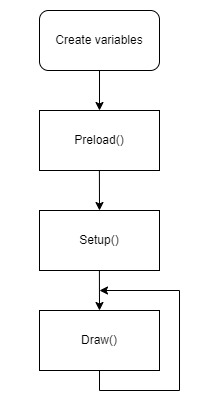
\includegraphics[width=1.7in]{block_diagram.jpg}
	\caption{Block diagram representing loading and servicing page.\label{fig:block_diagram}}
\end{figure}

\par
The block diagram presented in Fig.\ref{fig:block_diagram} shows the order of function calls. All three are based on p5.js library. Preload() is used to load assets used on the page. After all required files are loaded, a flag is raised to communicate with the Draw() function. Setup() is called directly after Preload() and initializes all the classes, as well as sets the frame rate and distance between obstacles.

\par
Draw() function waits for the flag from Preload() and Setup() completion. After both conditions are met, it calls custom-made functions which handle gameplay and window changes.

\subsection{Collision Object}

Collision object class handles obstacles stored in an array. It consists of variables responsible for current state and position of pylons and pickups if this option is turned on.

\par
This class provides methods for checking collision with player, as well as for moving and rendering obstacles in the current frame. Those methods are called from Game.js for each object in the array, creating a way to keep many obstacles on screen at the same time. It is also responsible for deleting objects which are outside the screen to prevent memory leaks.

\par
Height and position of passable part of an obstacle are generated randomly with rand() function. It is customized to have a different range, depending on the size of the user's screen.

\par
Additional pickups are also handled by this class. A special boolean variable is used to determine if the object should contain bonus points. Collision and rendering is handled by methods described above.

\begin{figure}
	\centering
	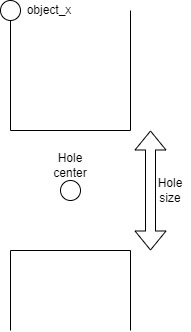
\includegraphics[width=2.3in]{obstacle_coords.jpg}
	\caption{Representation of Collision object class coordinates.\label{fig:collision}}
\end{figure}

\par
Fig.\ref{fig:collision} represents variables which are used to render and move obstacles. Computations are based on three presented values and screen size to accommodate different window sizes. If the option responsible for additional points is turned on, then a pickup is placed based on hole center value. Each object contains two boolean values responsible for giving points to the player and generating pickups.

\subsection{Handling switching between options}
To reduce usage of additional libraries, option handling was made with just JavaScript. Each window is represented by a div containing specific buttons, inputs and additional information. A file called div\textunderscore master.js manages the structure of those divs by changing the CSS property responsible for element visibility and style. After switching windows, a special function is called, hiding all divs which aren't required. Values such as user input are reset as well.

\par
Expanding this structure to handle more divs requires a future developer to edit a function called div\textunderscore create\textunderscore all() and add a new one responsible for handling the newly created div. Creation of this new element should be handled in the same file as well. A representation of current div structure can be seen in Fig.\ref{fig:div_handling}.

\par
Controlling sound volume and gameplay customization options is handled by functions in div\textunderscore create\textunderscore all() as well. Sounds can have two states, muted (default) and unmuted. When a user mutes a soundtrack, the song isn't stopped, but silenced.

\newpage

\vspace*{0.5in}

\begin{figure}
	\centering
	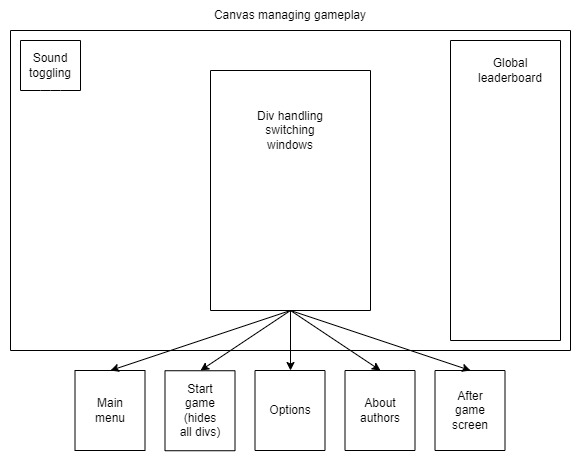
\includegraphics[width=5in]{div_handling.jpg}
	\caption{Representation of divs connection.\label{fig:div_handling}}
\end{figure}

\vspace*{0.5in}

\subsection{Laser obstacle}
The concept of laser element was overhauled few times during development. The final design decision was to make the laser remove one point for each frame the player touches it. The lowest score is capped at 0 to prevent negative values. Animation of firing is made based on font awesome icons and CSS "-webkit-mask-image" property to add overlay on the base laser.

\begin{figure}
	\centering
	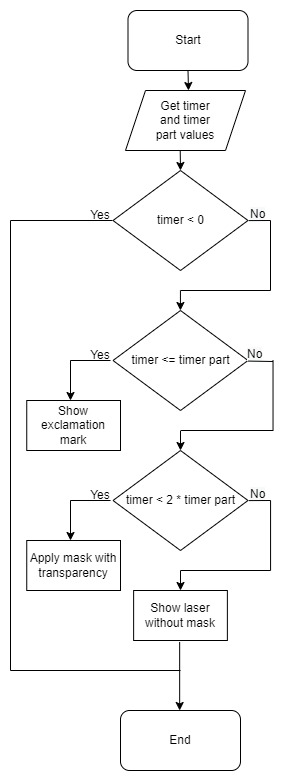
\includegraphics[width=3in]{laser.jpg}
	\caption{Block diagram representing process of laser rendering.\label{fig:laser}}
\end{figure}

\par
Future changes of laser style could be made by changing laser.css file, which contains gradient property describing laser appearance. By changing parameters in laser.js file, the future developer could edit animations speed and the time the laser is present on the screen. Fig.\ref{fig:laser} shows the algorithm used to render the laser firing animation.

\subsection{Image rendering}
Achieving parallax effect with background assets was crucial. To achieve this, two classes were made. Image\textunderscore rendering.js receives four parameters. Three of them are assets to produce the effect of randomly generated background. Fourth one is speed value. Background is divided into four main parts, all of them have different speed, which creates the desired effect.

\par
Image\textunderscore render.js handles changing coordinates for the asset it contains. To simplify code in Image\textunderscore rendering.js it creates three entities of Image\textunderscore render.js and manages them.

\par
Player character, pickups and obstacles images are handles in separate files. Each asset is characterized by a set of coordinates which changes each frame. Some of them were created using free packages shared online \cite{Facade009} \cite{Kitbash}.

\par
We've decided to use Midjourney AI\cite{Midjourney} for creation of backgrounds and some assets. The rest of the assets were created using Blender\cite{Blender}.

\subsection{CSS options}
To keep files managing clear, each distinct CSS option is handled in a separate file. For editing style of specific element, developer would have to find respective file and change properties of main element. As inspiration for part of our designs, we've used YouTube tutorials showcasing "Cyberpunk" themed creations \cite{CyberpunkCSS} \cite{GlitchCSS}.

\par
Some animations use root variables, which are changed through JavaScript. They are placed in a specific root.css file.

\section{Server side}
Main computations and user experience are handled on the client side. Our server is responsible for managing proper hosting and communication by Ajax requests which control players' scores in our MySQL database.

\begin{figure}[!htb]
	\centering
	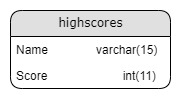
\includegraphics[width=2in]{database.jpg}
	\caption{Table responsible for handling inserted scores.\label{fig:database}}
\end{figure}

\par
We use database to handle only top scores of players. This meant that our database structure didn't have to be complex. Primary key was avoided as a deliberate choice, since only the best five scores are shown. Fig. \ref{fig:database} represents the table we've created.

\section{Problems during development}
During development, we've encountered several problems. Firstly, we've had to rewrite the physics system after implementing more complex images. This was caused by change in coordinates inputs for new functions and methods we use. Secondly, we've had to optimize generating obstacles and use a few tricks to make sure each resolution is served correctly. When using XAMPP as our temporary hosting on localhost, we've had few issues with page not refreshing correctly after implementing changes. This forced us to remove cookies and fully restart the page, which added some unwanted time during development.

\chapter{Summary}
We are very satisfied with the result of our work. The application fully meets our design expectations. Graphic and sound design fits well with the gameplay loop we created. Using version control proved to be very useful during debugging and optimization stage. Creating a proper README.md for our GitHub page was an additional task we didn't foresee, however it allowed us to manage progress more clearly. To prove usage of version control system, we submit a link to our GitHub page, which can be found \underline{\href{https://github.com/RadziooT/Cyberventure}{here}.}

\par
Possible future project expansions are:
\begin{itemize}
	\item adding additional gameplay mechanics such as increasing obstacle speed based on players score
	\item expanding leaderboard to contain separate tables for different configurations of customization options and changing global leaderboard from permanent top score to one being shown only for a specific amount of time
\end{itemize}

\par
To summarize, during our project we've gained valuable experience in handling multiple programming tools at the same time, which is sure to be useful in our future learning. It can also help us get a job as it is a valuable portfolio piece. We've also experienced working as a team and improved our abilities to divide and manage tasks properly.

%%%%%%%%%%%%%%%%%%%%%%%%%%%%%%%%%%%%%%%%%%%%%%%%%%%%%%%%%%%%%%%%%
%% BIBLIOGRAPHY.
%%%%%%%%%%%%%%%%%%%%%%%%%%%%%%%%%%%%%%%%%%%%%%%%%%%%%%%%%%%%%%%%%

\newpage
\phantomsection
\addcontentsline{toc}{chapter}{Bibliography}

\bibliographystyle{IEEEtran} % IEEE bibliographic/citation style.
\bibliography{IEEEfull,it-bib}

\newpage
\phantomsection

\appendix
\chapter{Early development and graphic designs}

\begin{figure}[!htb]
	\centering
	
\includegraphics[width=2in]{Appendix/first_stage.jpg}
	\caption{First stage of development with working gameloop}
\end{figure}

\begin{figure}[!htb]
	\centering
	
\includegraphics[width=1in]{Appendix/player.png}
	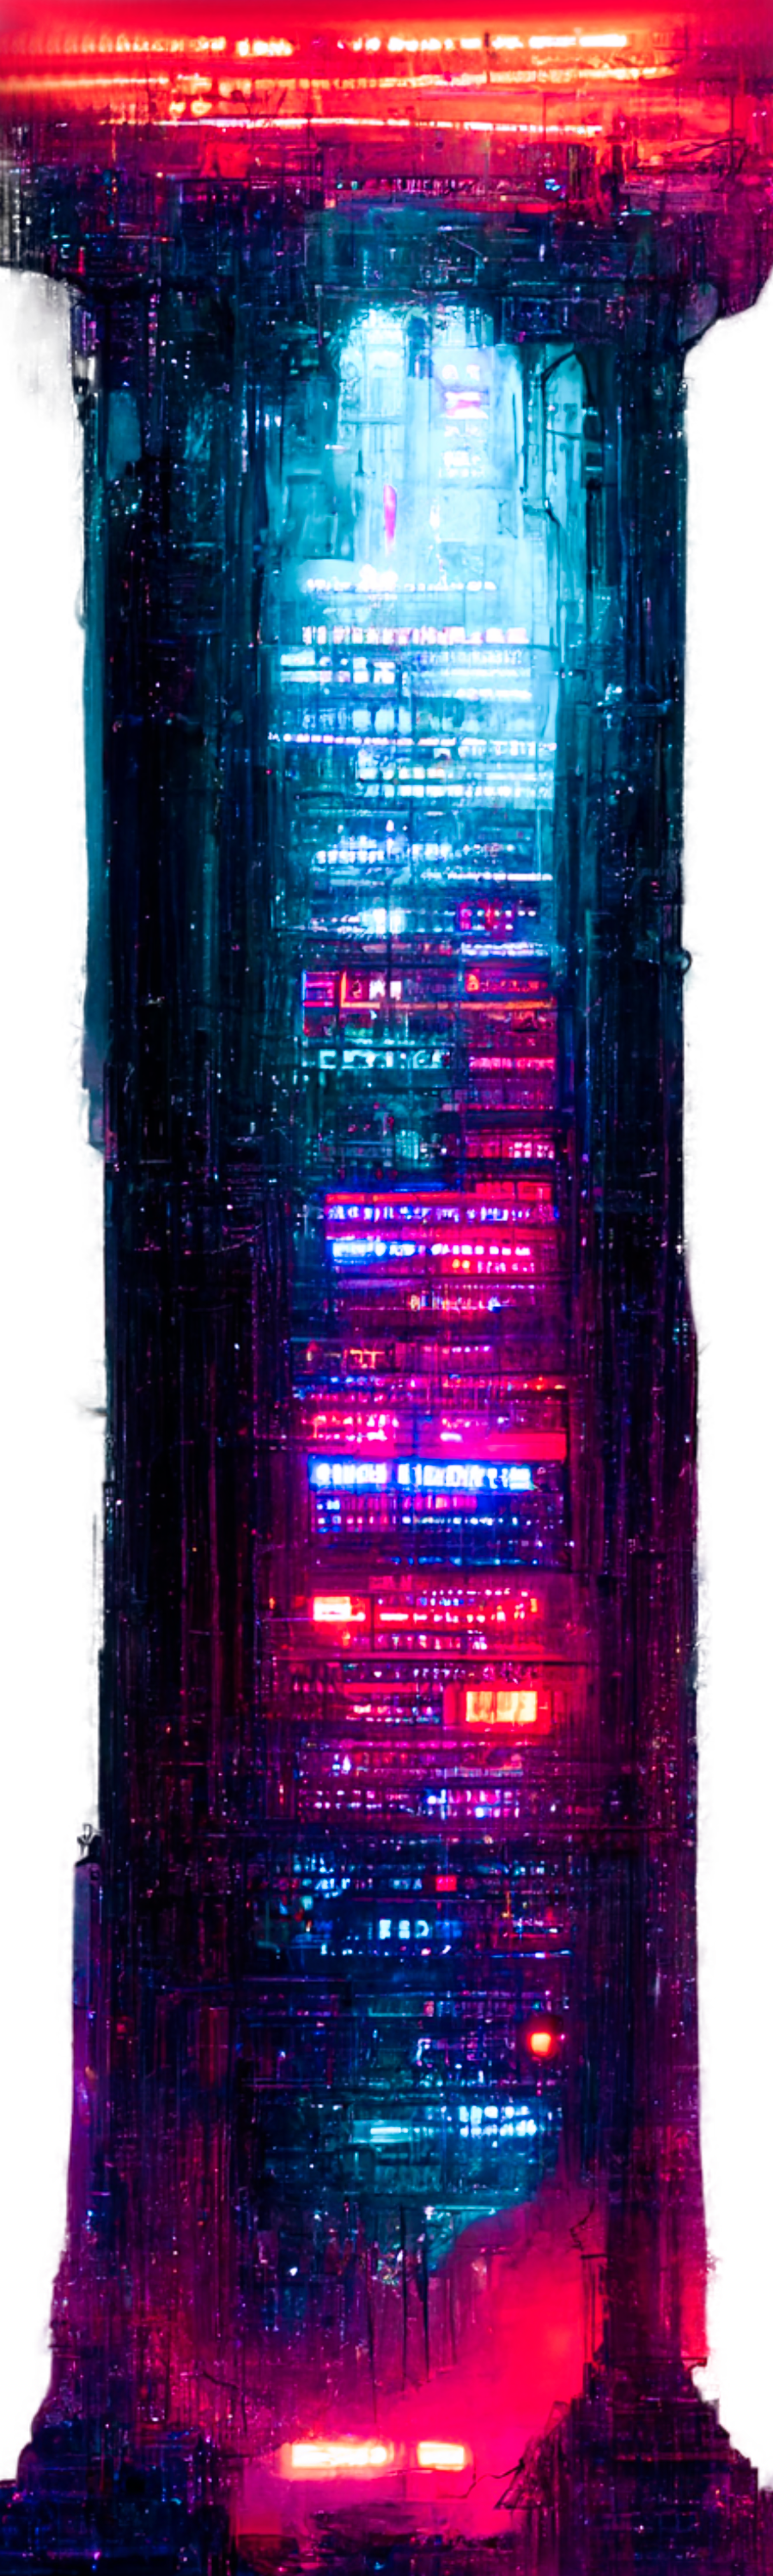
\includegraphics[width=1in]{Appendix/obstacle.png}
	\caption{Final player and obstacle designs}
\end{figure}

\begin{figure}
	\centering
	
\includegraphics[width=2in]{Appendix/volume.png}
	\caption{Two states of volume icon, animation was added to toggle between them}
\end{figure}

\begin{figure}
	\centering
	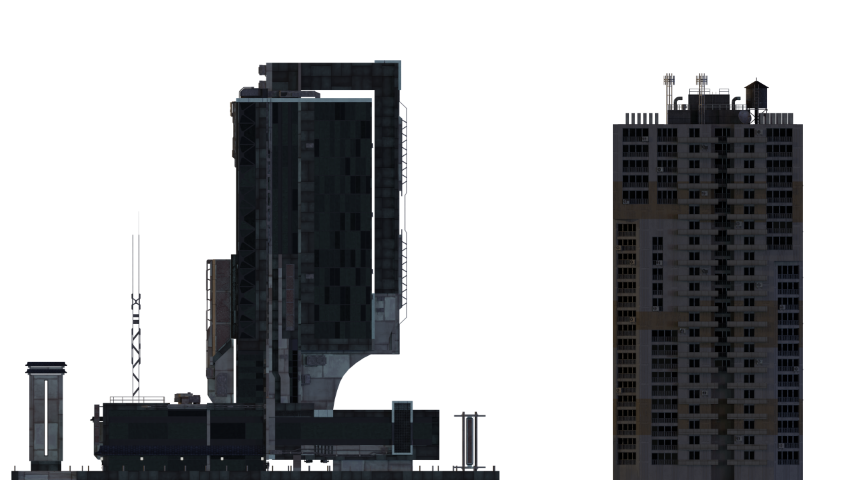
\includegraphics[width=2in]{Appendix/created_assets_1.png}
	
\includegraphics[width=2in]{Appendix/created_assets_2.png}
	\caption{Assets used as part of background layering}
\end{figure}

\newpage

\begin{figure}
	\centering
	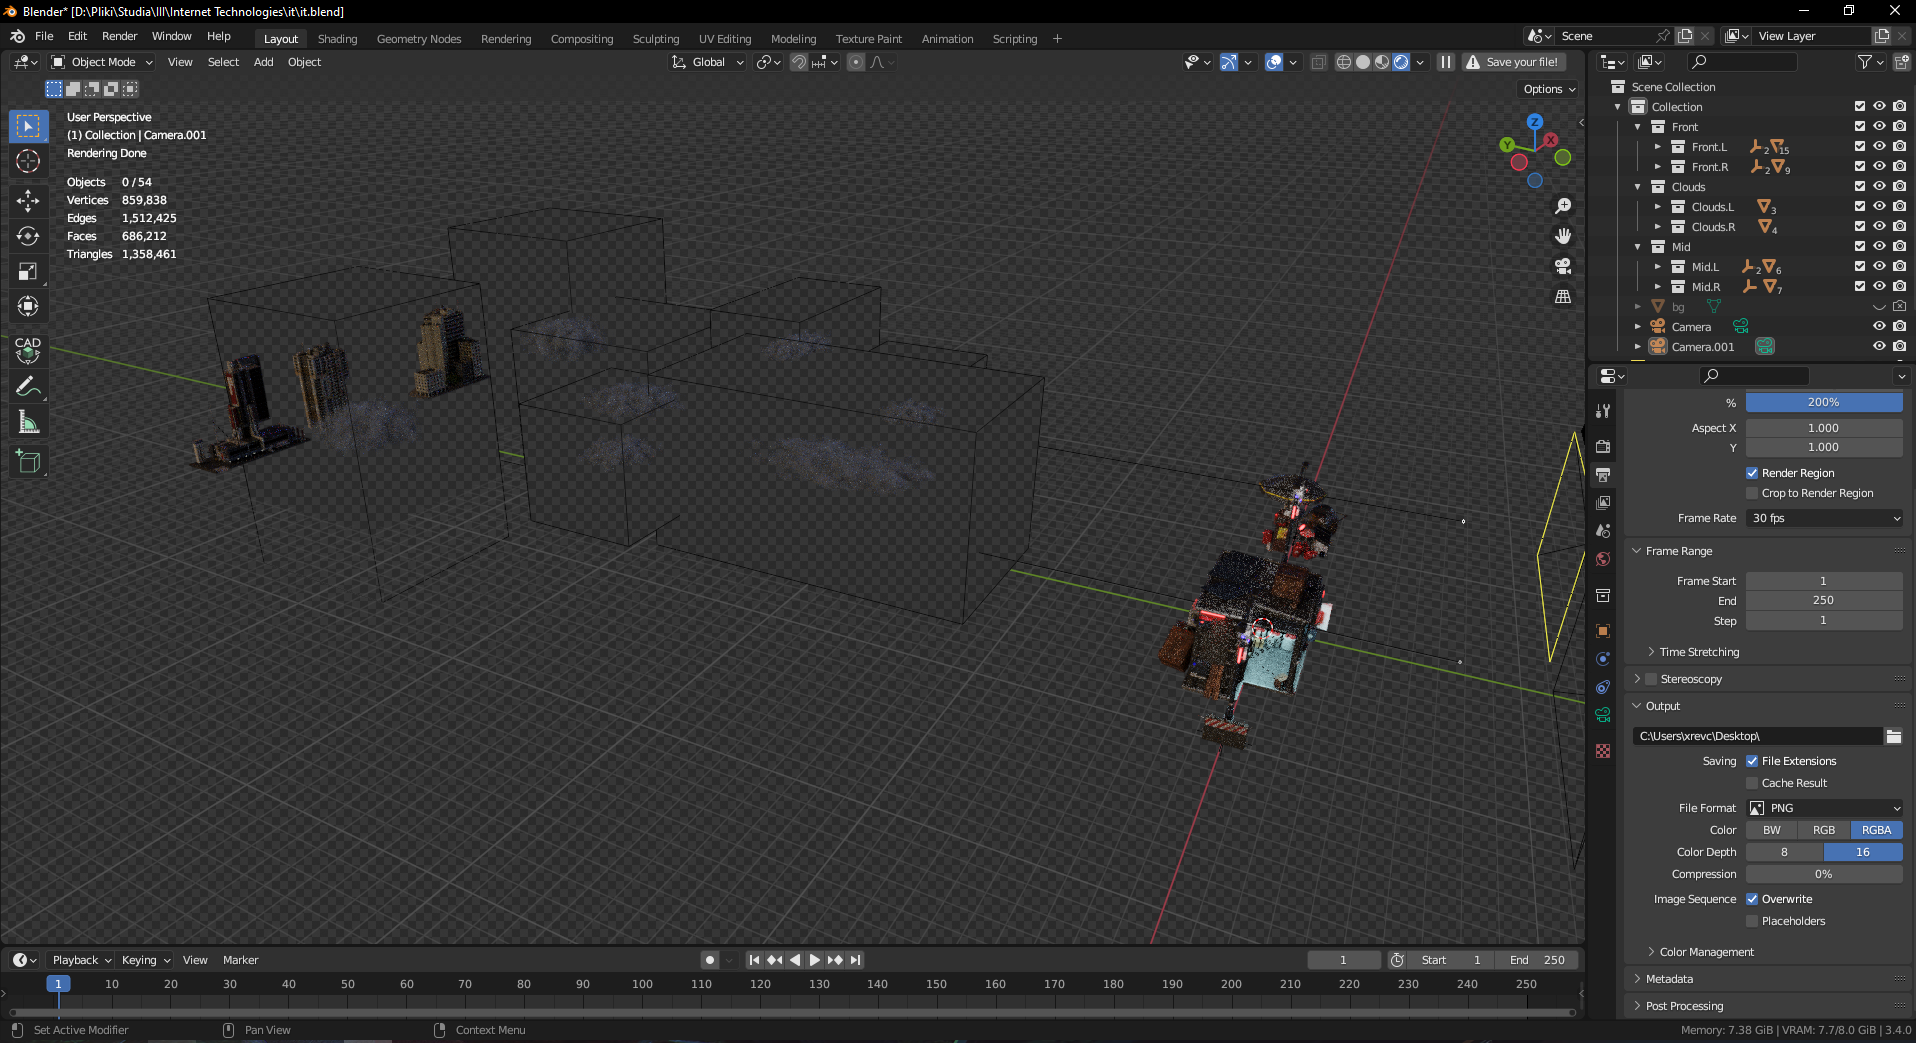
\includegraphics[width=0.9\textwidth]{Appendix/Blender_1.png}
	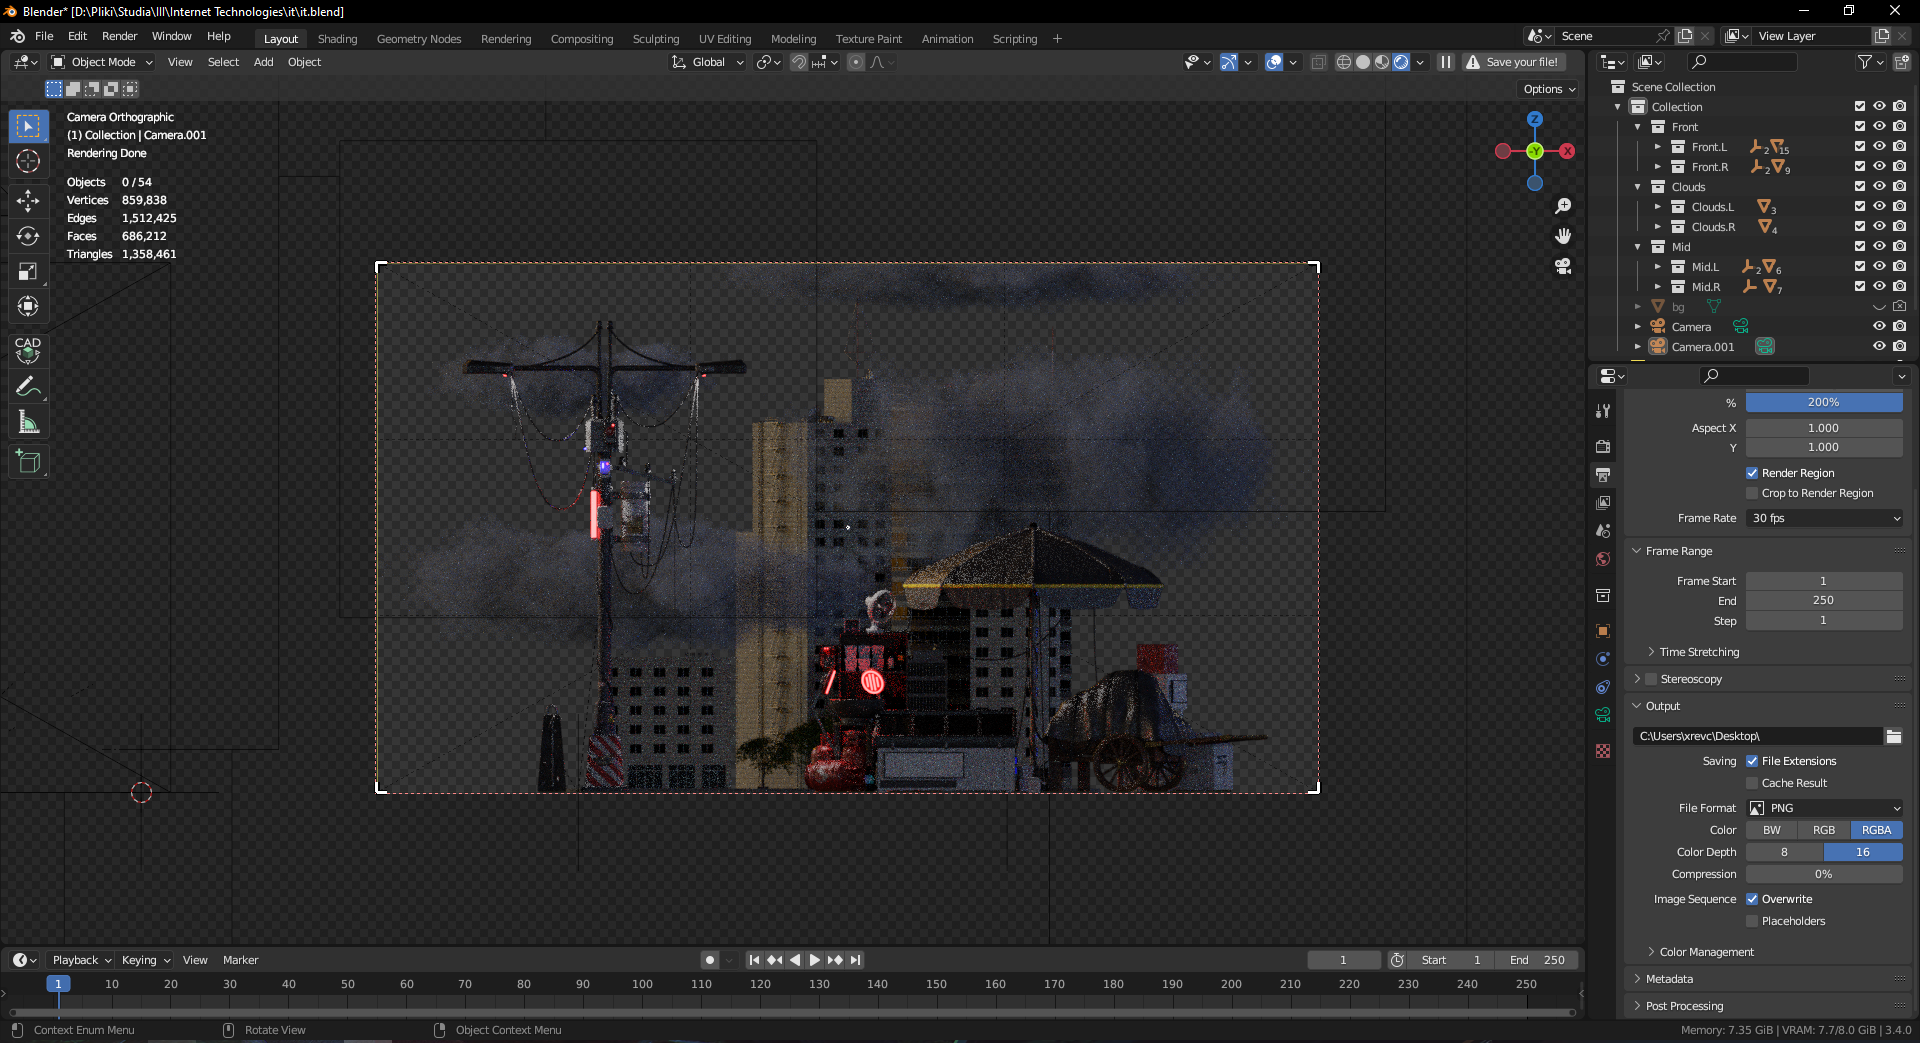
\includegraphics[width=0.9\textwidth]{Appendix/Blender_2.png}
	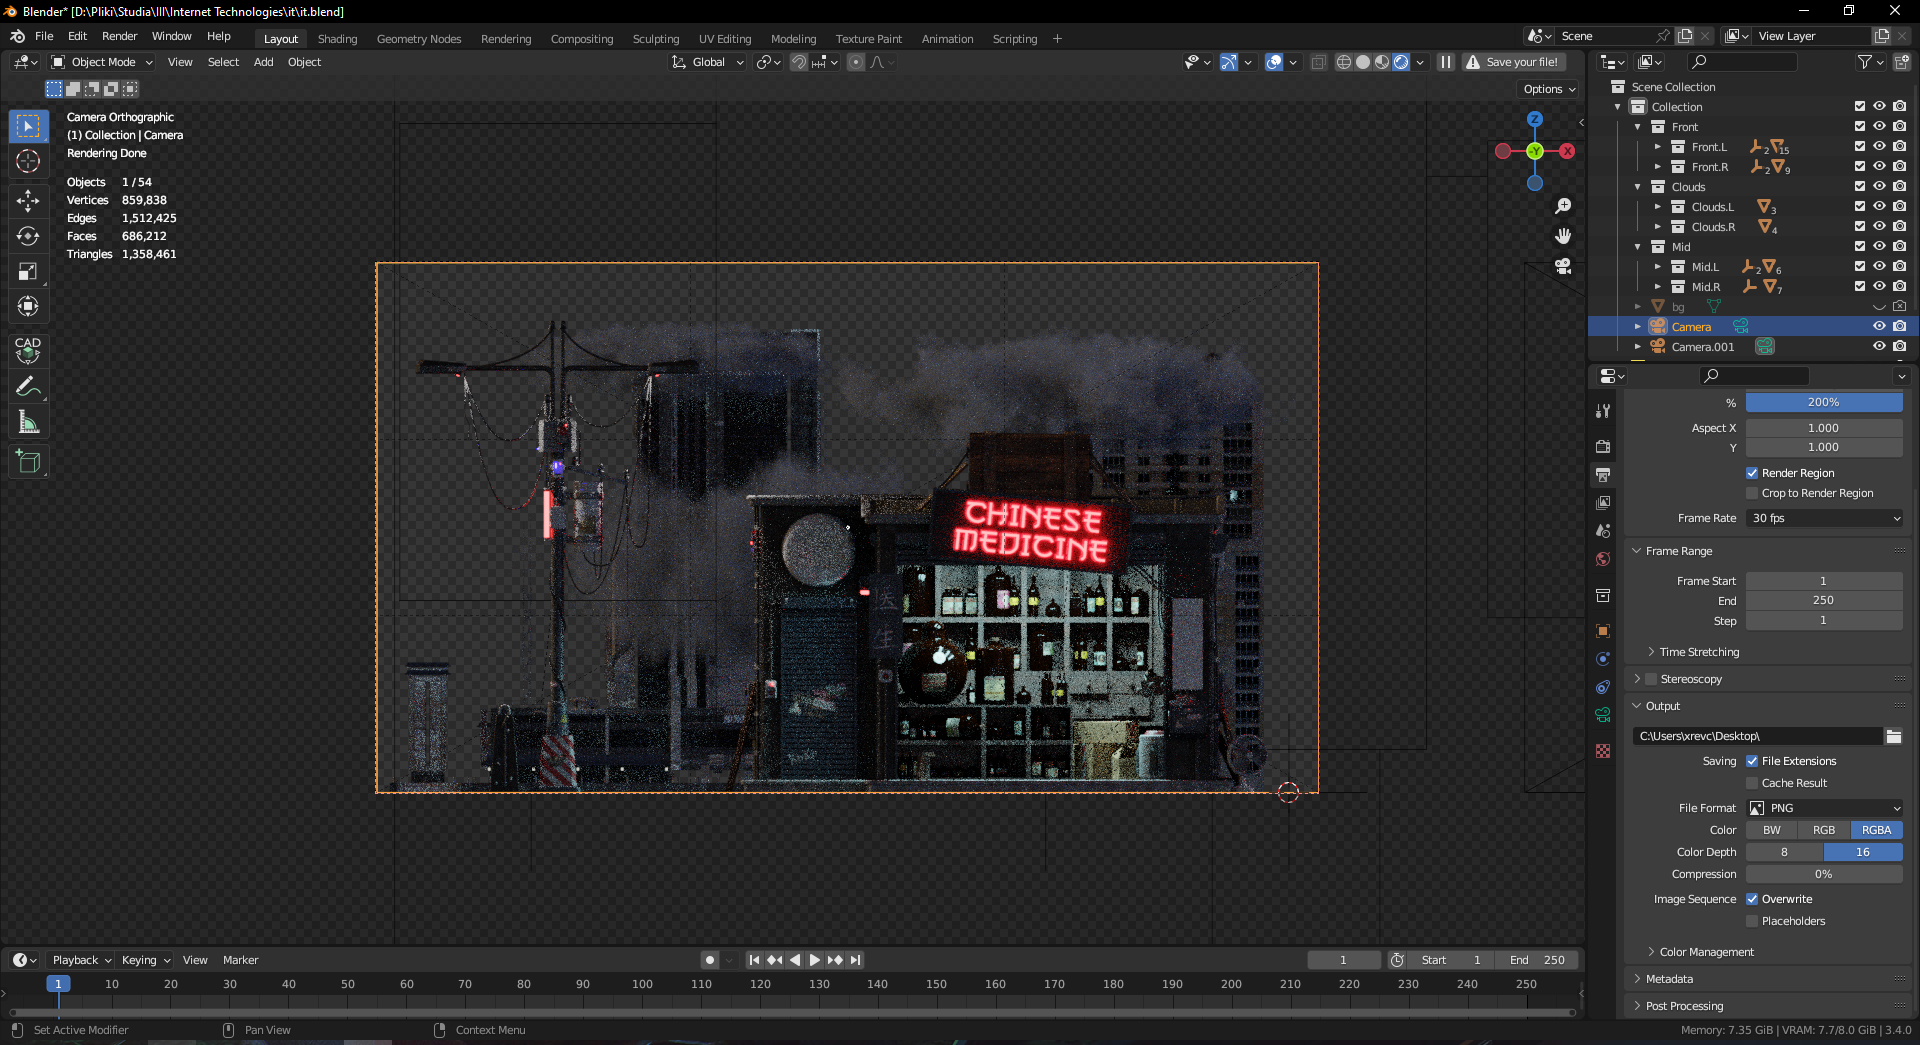
\includegraphics[width=0.9\textwidth]{Appendix/Blender_3.png}
	\caption{Creation process of 3D assets}
\end{figure}

\end{document}